\documentclass{article}
\usepackage[utf8]{inputenc}
\usepackage{amsmath}
\usepackage{amsthm}
\usepackage[left=1in,right=1in,top=1in,bottom=1in]{geometry}
\usepackage{graphicx}
\usepackage{float}
\usepackage{titling}
\usepackage{algorithm}
\usepackage[noend]{algpseudocode}
\usepackage[numbib,nottoc]{tocbibind}
\usepackage{indentfirst}


\setlength{\droptitle}{-1.5cm}

\newcounter{heuristic} \setcounter{heuristic}{0}
\renewcommand{\theheuristic}{\Alph{heuristic}}

\newenvironment{heuristic}[1]%
{
\refstepcounter{heuristic}
\subsection*{Heuristic \theheuristic}
}%
{}

\makeatletter
\def\BState{\State\hskip-\ALG@thistlm}
\makeatother

\title{Vertex Coloring and Applications}
\date{May 5, 2017}
\author{Shawn Seymour\\ University of Minnesota Morris}

\newtheorem{prop}{Proposition}
\newtheorem{theorem}{Theorem}

\theoremstyle{definition}
\newtheorem{definition}{Definition}

\begin{document}

\maketitle

\setlength{\parskip}{0.3cm}

\section{Introduction}
Consider the map of the 48 contiguous states in the USA. Suppose we would like to color each state such that no two states that share a boundary have the same color. How many colors would it take to do this? This problem can be modeled as a \emph{graph}. In general, we could represent every state with a \emph{vertex} and draw an \emph{edge} between two states that share a border. A graph, denoted $G = (V, E)$, is a set of vertices $V$ and a set of edges $E$. A \emph{simple graph} is a loopless, undirected graph where no two edges connect the same pair of vertices. For our purpose, assume all graphs are simple graphs. This problem, along with many others, can be solved using vertex coloring.

\begin{figure}[H]
\centering
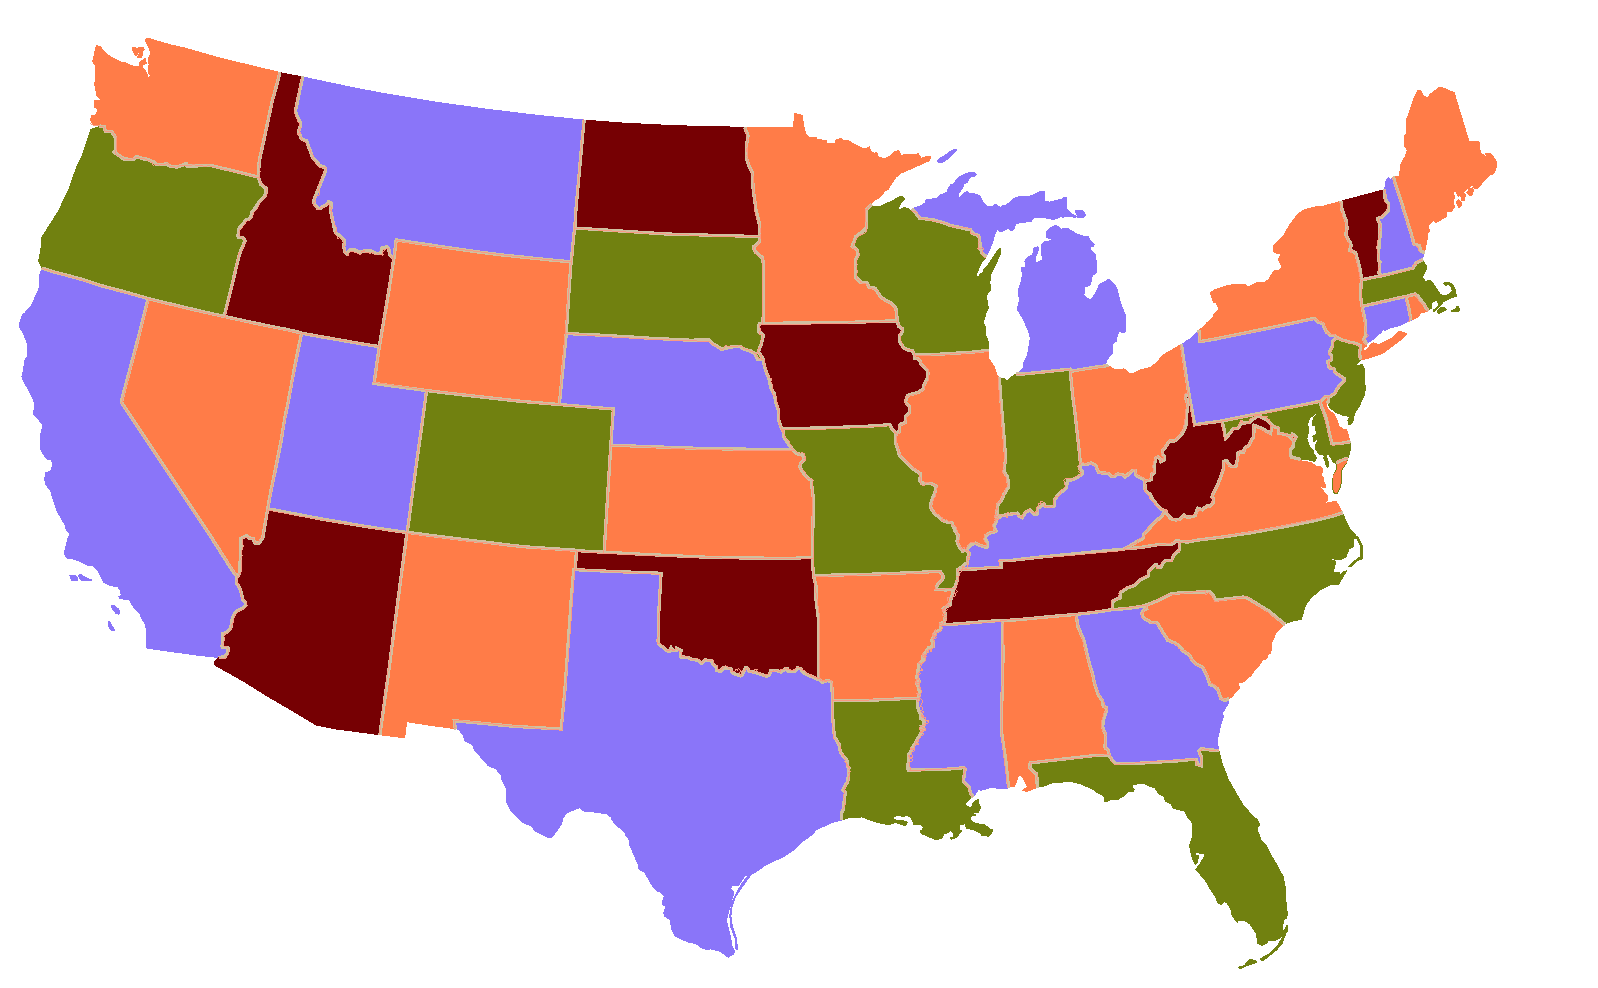
\includegraphics[width=0.5\linewidth]{figures/map-colors.pdf}
\caption{A proper coloring of the USA}\label{fig:map}
\end{figure}

A \emph{vertex coloring} of a graph $G$ is an assignment of colors to each vertex of a graph. A \emph{proper vertex coloring} assigns colors to a graph $G$ such that no two adjacent vertices share the same color. This can be described as a function $f : V \rightarrow S = \{1, 2, \ldots, k\}$ such that $\forall u,w \in V$, if $(u,w) \in E$, then $f(u) \neq f(w)$. Note that this constraint is the same constraint we applied to our map example. This means we could color our map according to our constraint with a proper vertex coloring.

The \emph{chromatic number}, denoted $\chi(G)$, is the minimum number of colors needed to have a proper vertex coloring of a graph $G$. The \emph{vertex coloring problem} (VCP), when given a graph $G$, is to find $\chi(G)$. By applying the vertex coloring problem to our map example, we can determine how many colors one would need to color it with regards to our constraint. As it turns out, it only takes \emph{four} colors to properly color the map of the USA. This is shown in Figure \ref{fig:map}.


\newpage

\bibliographystyle{abbrv}
\bibliography{references}


\end{document}
